\chapter{再入段运动特性分析与弹道设计}
\thispagestyle{empty}

\section{再入段运动方程}

\subsection{矢量形式段动力学方程}

空间质心运动方程段矢量形式为
\begin{equation}
	m \dfrac{\d^2 \bm{r}}{\d t^2} = \bm{P} + \bm{R} + \bm{F}_{c} +m\bm{g} + \bm{F}'_k
\end{equation}
由于再入段不考虑推力、控制力及附加哥氏力(无质量变化)等作用,则质心运动矢量方程为
\begin{equation}
	m \dfrac{\d^2 \bm{r}}{\d t^2} = \bm{R} + m\bm{g}
\end{equation}

在体坐标系中建立的绕质心动力学方程为
\begin{equation}
	\bm{I}\cdot \dfrac{\d \bm{\omega}_T}{\d t} + \bm{\omega}_T\times(\bm{I}\cdot \bm{\omega}_T) = \bm{M}_{st} + \bm{M}_c + \bm{M}_d + \bm{M}'_k+\bm{M}'_{rel}
\end{equation}
当不考虑控制力矩、附加哥氏力矩(无质量变化)等作用时,矢量方程为
\begin{align}
	\bm{I}\cdot \dfrac{\d \bm{\omega}_T}{\d t} + \bm{\omega}_T\times(\bm{I}\cdot \bm{\omega}_T) &= \bm{M}_{st} + \bm{M}_d \\
	\bm{\omega}_T = \bm{\omega} + \bm{\omega}_e
\end{align}
其中,$\bm{\omega}$为飞行器姿态相对于发色坐标系的转动角速度,$\bm{\omega_e}$为地球自转角速度。


\subsection{地面发射坐标系中再入段空间运动方程}
可将矢量运动方程分解到发射系中,也可直接利用空间运动方程进行简化得到:

\noa[1] 无动力,推力为0。
\begin{equation}
	P = 0
\end{equation}

\noa[2] 无控制,不考虑控制偏转角及控制力。
\begin{align}
	X_{\text{1\c}} = Y_{2\c} = Z_{3\c} = 0\\
	\delta_\varphi = \delta_\psi = \delta_\gamma = 0
\end{align}

\noa[3] 无质量消耗,为理想的常质量质点系。
\begin{align}
	\dot{m} &= 0 \\
	\dot{I}_{x1} = \dot{I}_{y1} &= \dot{I}_{z1} = 0
\end{align}

\noa[4] 飞行时间短,可忽略地球自转对相对角速率对影响。
\begin{equation}
	\begin{bmatrix}
		\omega_{Tx1} \\
		\omega_{Ty1}\\
		\omega_{Tz1}
	\end{bmatrix}
	=
	\begin{bmatrix}
		\omega_{x1} \\
		\omega_{y1} \\
		\omega_{z1}
	\end{bmatrix}
	\qquad 
	\begin{bmatrix}
		\varphi_T \\
		\psi_T \\
		\gamma_T
	\end{bmatrix}
	=
	\begin{bmatrix}
		\hspace*{0.1em}\varphi \hspace*{0.1em}\\
		\hspace*{0.1em}\psi \hspace*{0.1em}\\
		\hspace*{0.1em}\gamma \hspace*{0.1em}
	\end{bmatrix}
\end{equation}
则得到简化后的22个方程为
\begin{equation}
	\begin{cases}
		\, m 
		\begin{bmatrix}
			\dfrac{\d v_x}{\d t} \\[0.5em]
			\dfrac{\d v_y}{\d t} \\[0.5em]
			\dfrac{\d v_z}{\d t}
		\end{bmatrix}
		= G_V
		\begin{bmatrix}
			-X\\
			Y \\
			Z
		\end{bmatrix}
		+ m \dfrac{\dot{g}_r}{r}
		\begin{bmatrix}
			x  + R_{ox} \\
			y + R_{oy} \\
			z + R_{oz}
		\end{bmatrix}
		+ m \dfrac{g_{\omega e}}{\omega_e}
		\begin{bmatrix}
			\omega_{ex} \\
			\omega_{ey} \\
			\omega_{ez}
		\end{bmatrix}
		- m
		\begin{bmatrix}
			a_{11} & a_{12} & a_{13} \\
			a_{21} & a_{22} & a_{23} \\
			a_{31} & a_{32} & a_{33}
		\end{bmatrix}
		\begin{bmatrix}
			x  + R_{ox} \\
			y + R_{oy} \\
			z + R_{oz}
		\end{bmatrix}
		 - m
		 \begin{bmatrix}
		 	b_{11} & b_{12} & b_{13} \\
		 	b_{21} & b_{22} & b_{23} \\
		 	b_{31} & b_{32} & b_{33}
		 \end{bmatrix}
	 	\begin{bmatrix}
	 		v_x \\
	 		v_y \\
	 		v_z
	 	\end{bmatrix} 
 	\\[4em]
 	
 	\,  
 	\begin{bmatrix}
 		I_{x1} \dfrac{\d \omega_{x1}}{\d t} \\[0.5em]
 		I_{y1} \dfrac{\d \omega_{y1}}{\d t} \\[0.5em]
 		I_{z1} \dfrac{\d \omega_{z1}}{\d t}
 	\end{bmatrix}
 	+ 
 	\begin{bmatrix}
 		\big(I_{z1} - I_{y1}\big)\omega_{z1}\omega_{y1} \\
 		\big(I_{x1} - I_{z1}\big)\omega_{x1}\omega_{z1} \\
 		\big(I_{y1} - I_{x1}\big)
 	\end{bmatrix}
 	=
 	\begin{bmatrix}
 		0 \\
 		m_{y1\st}q S_M l_K \\
 		m_{z1\st}q S_M l_K 
 	\end{bmatrix}
 	+
 	\begin{bmatrix}
 		m_{x1}^{\overline{\omega}_{x1}}q S_M l_K\overline{\omega}_{x1}\\
 		m_{y1}^{\overline{\omega}_{y1}}q S_M l_K\overline{\omega}_{y1}\\
 		m_{z1}^{\overline{\omega}_{z1}}q S_M l_K\overline{\omega}_{z1}
 	\end{bmatrix}
 	\\[4em]
 	
 	\, 
 	\begin{bmatrix}
 		\dfrac{\d x}{\d t} \\[0.5em]
 		\dfrac{\d y}{\d t} \\[0.5em]
 		\dfrac{\d z}{\d t} 
 	\end{bmatrix}
	=
	\begin{bmatrix}
		v_x \\
		v_y \\
		v_z
	\end{bmatrix}
	\\[4em]
	
	\, 
	\begin{bmatrix}
		\omega_{x1} \\
		\omega_{y1} \\
		\omega_{z1}
	\end{bmatrix}
	=
	\begin{bmatrix}
		\dot{\gamma} - \dot{\varphi}\sin \psi \\
		\dot{\varphi}\cos \gamma + \dot{\varphi}\cos \psi \sin \gamma \\
		\dot{\varphi}\cos \psi \cos \gamma - \dot{\psi}\sin \gamma
	\end{bmatrix}
	\\[3.5em]
	
	\,
	\begin{cases}
		\, \theta = \arctan \big(v_y/ v_x\big) \\
		\, \sigma = - \arcsin(v_z /v)
	\end{cases}
	\\[2em]
	
	\,
	\begin{cases}
		\, \sin \beta = \cos\big(\varphi - \theta\big)\cos \sigma \sin \psi \cos \gamma + \sin \big(\varphi - \theta\big)\cos \sigma \sin \gamma - \sin \sigma \cos \psi \cos \gamma \\
		\, -\sin \alpha \cos \beta = \cos \big(\varphi - \theta\big)\cos \sigma \sin \psi \sin \gamma - \sin\big(\varphi - \theta\big) \cos \sigma \cos \gamma - \sin \sigma \cos \psi \sin \gamma \\
		\, \sin \nu = \dfrac{1}{\cos \sigma} \big(\cos \alpha \cos \psi \sin \gamma \big) - \sin \psi \sin \alpha 
	\end{cases}
	\\[3.2em]
	
	\, r = \sqrt{\big(x + R_{ox}\big)^2 + \big(y+R_{oy}\big)^2 + \big(z + R_{oz}\big)^2}
	\\[1em]
	
	\, \sin \phi = \dfrac{\big(x + R_{ox}\big)\omega_{ex} + \big(y + R_{oy}\big)\omega_{ey} + \big(z + R_{oz}\big)\omega_{ez}}{r\omega_e}
	\\[1em]
	
	\, R = \dfrac{a_e b_e}{\sqrt{a_e^2 \sin^2 \phi + b_e^2 \cos^2 \phi}}
	\\[1em]
	
	\, h = r - R
	\\
	
	v = \sqrt{v_x^2 + v_y^2 + v_z^2}
	\end{cases}
\end{equation}

\subsection{以总攻角、总升力表示的再入段空间弹道方程}

由于再入段飞行器可利用升力进行机动飞行,因此一些再入飞行器外形设计成升力体外形,不具有轴对称性,其法向气动力与横向气动力是不对称的。因此为充分利用升力体的机动能力,引入总升力与总攻角的概念。


\begin{figure}[!htb]
	\centering
	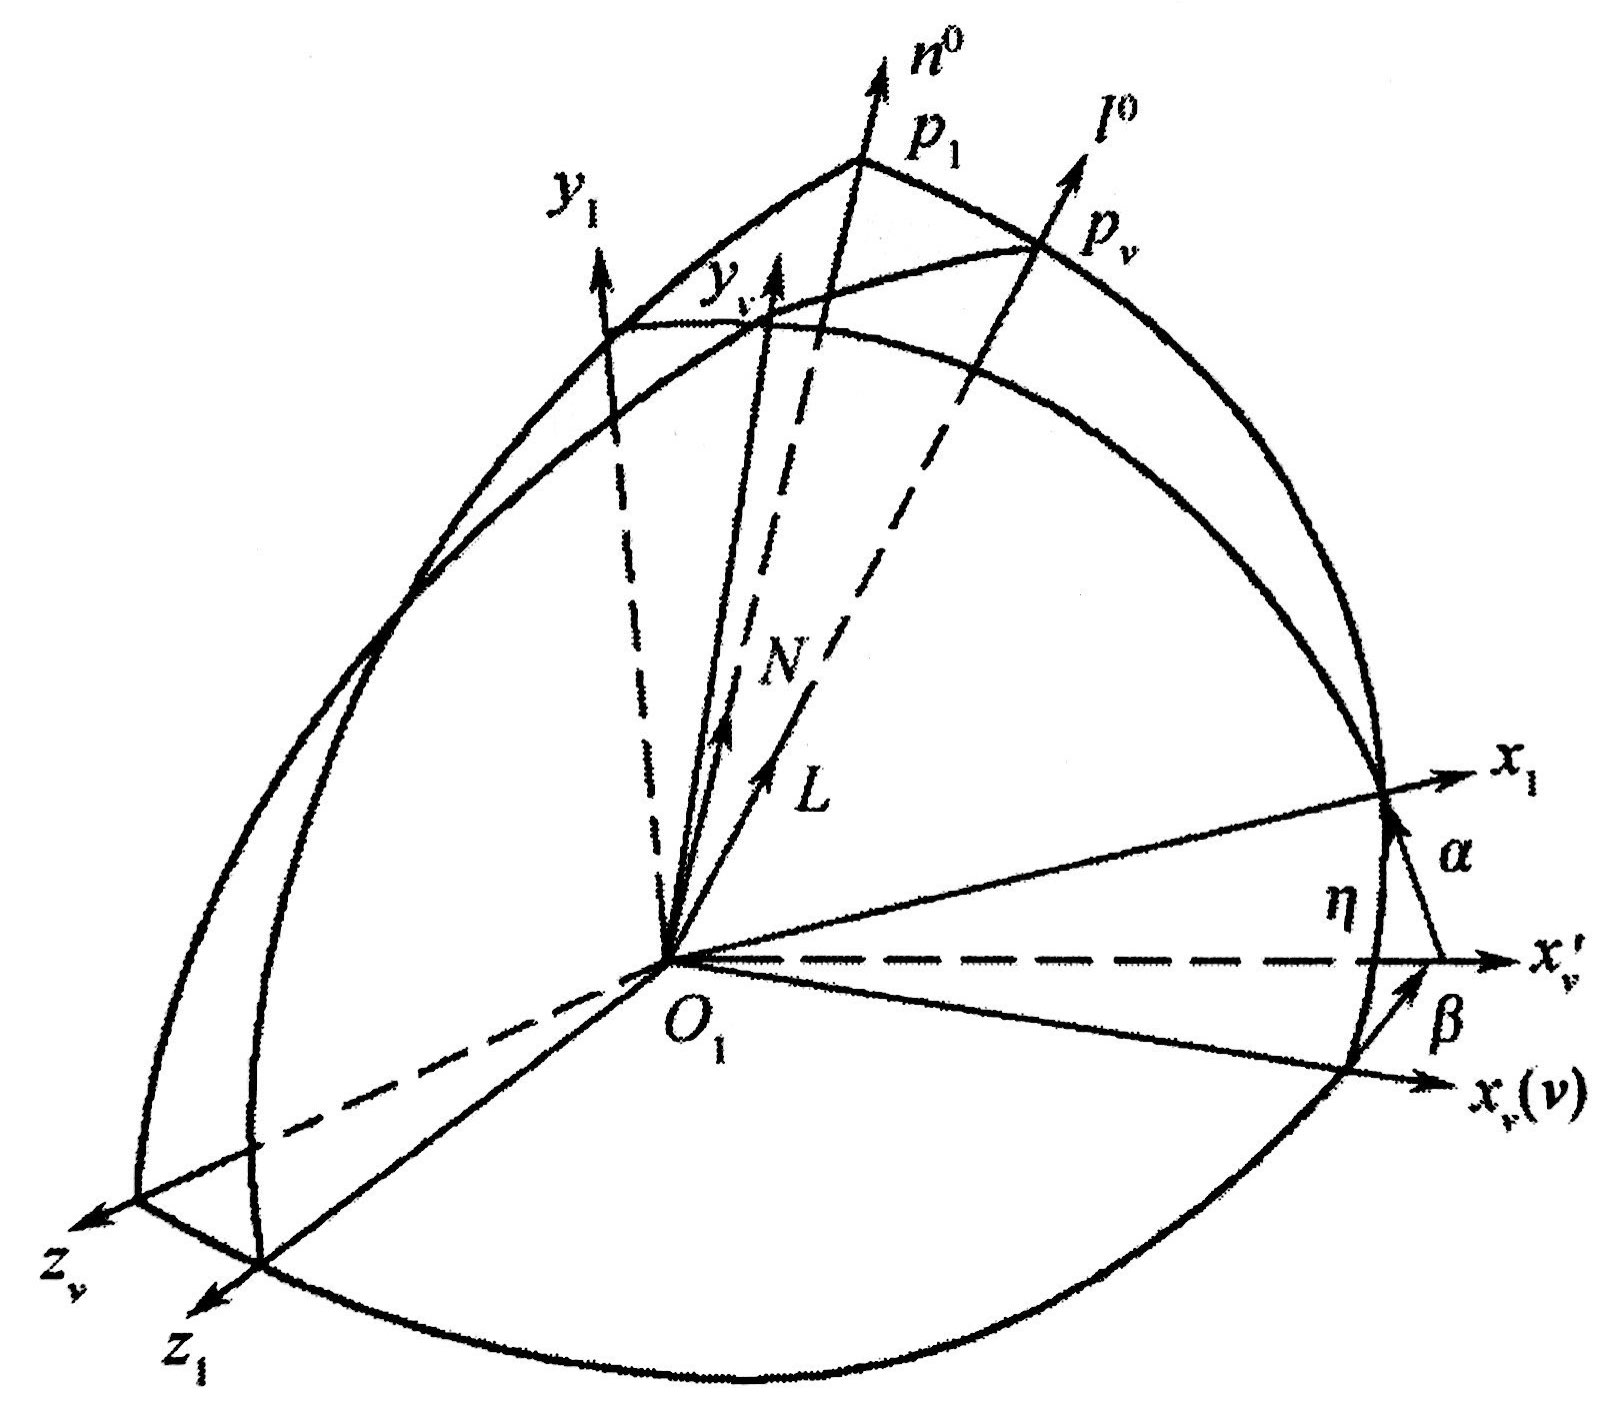
\includegraphics[width=0.4\linewidth]{pic/总攻角.jpg}
	\caption{总攻角$\eta$、总法向力$N$与总升力$L$}
	\label{总攻角}
\end{figure}

如图 \ref{总攻角} 所示,\dy[总攻角]{ZGJ}定义为速度轴$x_v$与弹体纵轴$x_1$的夹角,记作$\eta$,对应平面为总攻角平面。因此气动力可分解为
\begin{align}
	&\bm{R} = - X_1 \bm{x}_1^0 + N\bm{n}^0 \qquad \mbox{总法向力}N\mbox{垂直}\bm{x}_1\mbox{方向}\\
	&N\bm{n}^0 = Y_1\bm{y}_1^0 + Z_z \bm{z}_1^0 \qquad z_1o_1y_1\mbox{面与}x_1o_1x_v\mbox{面交线}O_1P_1
\end{align}

总攻角面内将气动力投影到速度系
\begin{align}
	&\bm{R} = - X\bm{x}_v^0 + L\bm{l}^0 \qquad \mbox{总法向力}N\mbox{垂直}\bm{x}_v\mbox{方向} \\
	&L\bm{l}^0 = Y \bm{y}_v^0 + Z \bm{z}_v^0 \qquad  z_vo_1y_v\mbox{面与}x_1o_1x_v\mbox{面交线}O_1P_v
\end{align}
下面给出引入总攻角后相关角度与力的相互关系:

\noa[1] 总攻角$\eta$与攻角$\alpha$、侧滑角$\beta$的关系
\begin{equation}
	\begin{cases}
		\, \cos \eta = \bm{x}_v^0 \cdot \bm{x}_1^0 \\
		\, \cos \alpha = \bm{x}_v^{'0}\cdot \bm{x}_z^0 \\
		\, \cos \beta = \bm{x}_v^0 \cdot \bm{x}_1^{'0}
	\end{cases}
\end{equation}
而速度轴与箭体轴之间存在转换关系,有
\begin{align*}
	\cos \eta &= \cos \alpha \cdot \cos \beta \\
	\sin^2 \eta &= \sin^2 \alpha + \sin^2 \beta - \sin^2 \alpha \sin^2 \beta 
\end{align*}
当攻角、侧滑角为小角度时,可以近似为
\begin{equation}
	\eta = \sqrt{\alpha^2 + \beta^2}
\end{equation}

\noa[2] 总法向力$N$与总升力$L$的关系

由于总法向力$N$和总升力$L$均在总攻角平面$x_1o_1x_v$内,则有
\begin{equation}
	\begin{cases}
		\, X = N \sin \eta + X_1 \cos \eta \\
		\, L = N \cos \eta - X_1 \sin \eta
	\end{cases}
\end{equation}

\begin{figure}[!htb]
	\centering
	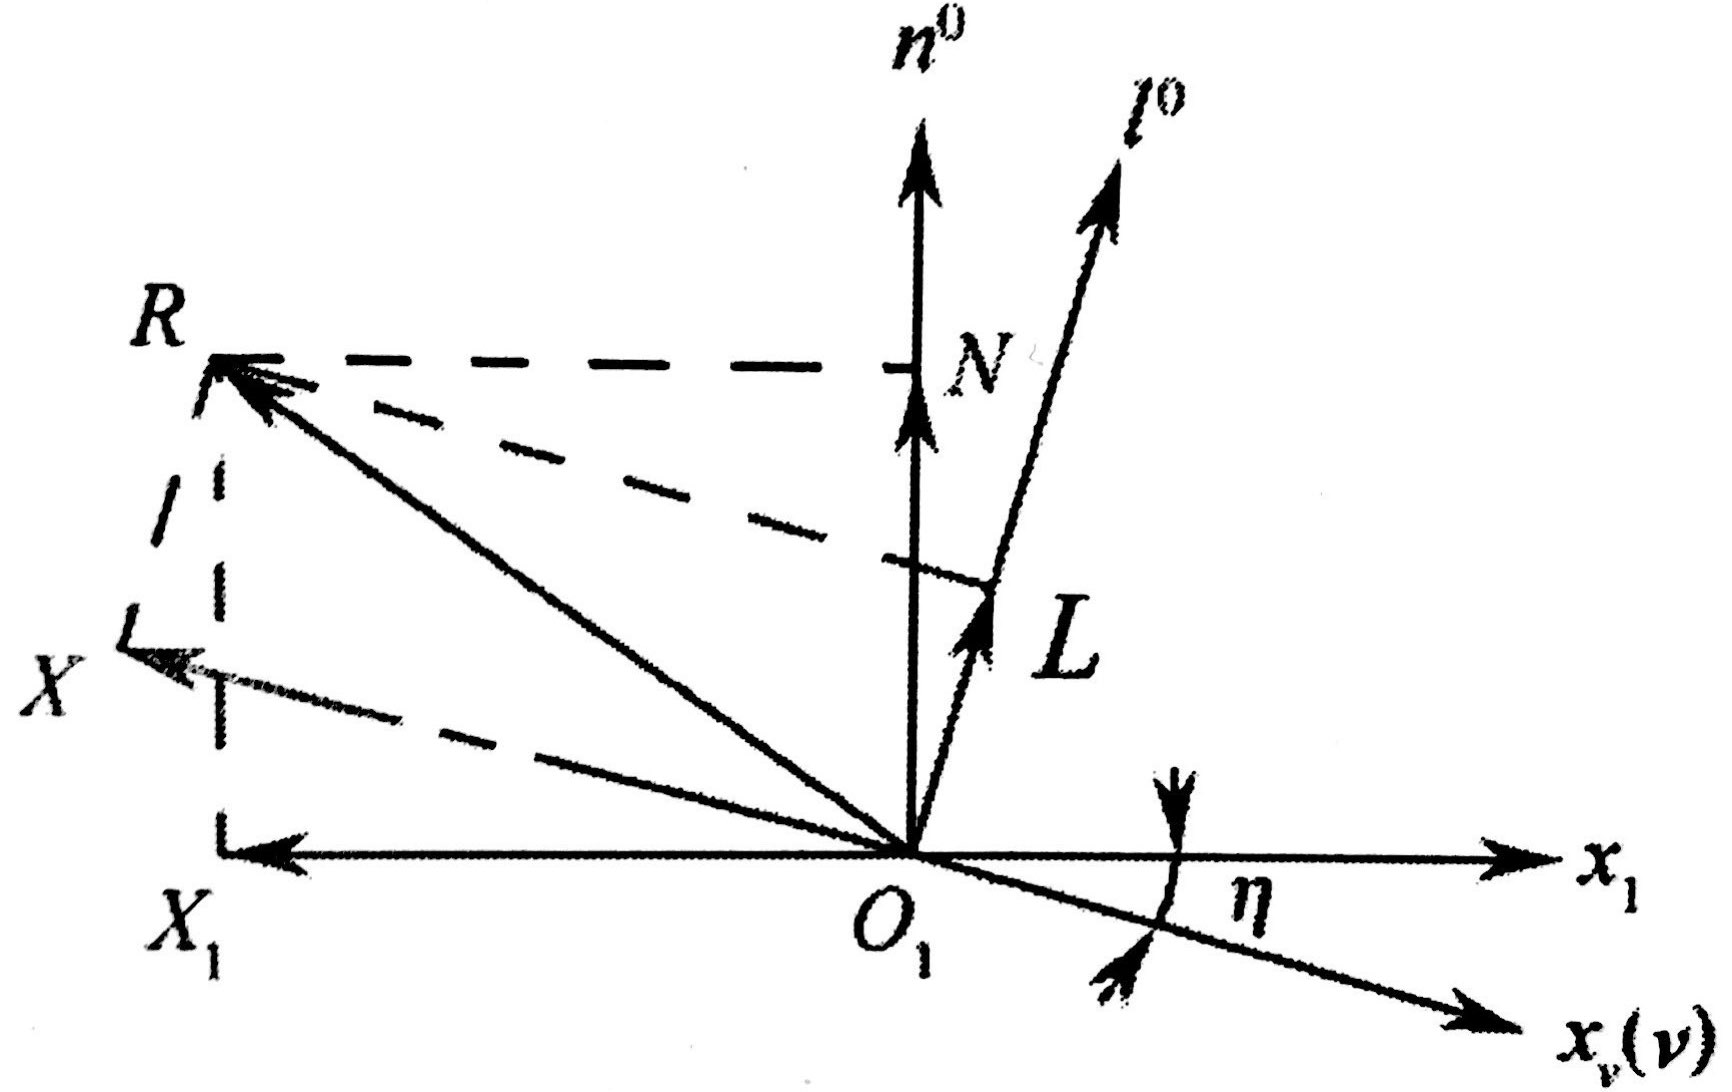
\includegraphics[width=0.4\linewidth]{pic/阻力.jpg}
	\caption{阻力$X$、总升力$L$与轴向力$X_1$、总法向力$N$的关系}
\end{figure}

若采用气动力系数描述,有
\begin{equation}
	\begin{cases}
		\, X = C_xqS_M \\
		\, X_1 = C_{x1} q S_M \\
		\, L = C_L q S_M \\
		\, N = C_N q S_M
	\end{cases}
	\quad \Longrightarrow \quad 
	\begin{cases}
		\, C_x = C_N \sin \eta + C_{x1} \cos \eta \\
		\, C_L = C_N \cos \eta - C_{x1} \sin \eta
	\end{cases}
\end{equation}
\red[注:有时候阻力系数可以用$C_D$表示,轴向力系数用$C_A$表示。]
\vspace*{0.5em}

\noa[3] 总法向力$N$与法向力$Y_1$、横向力$Z_1$关系
\begin{figure}[!htb]
	\centering
	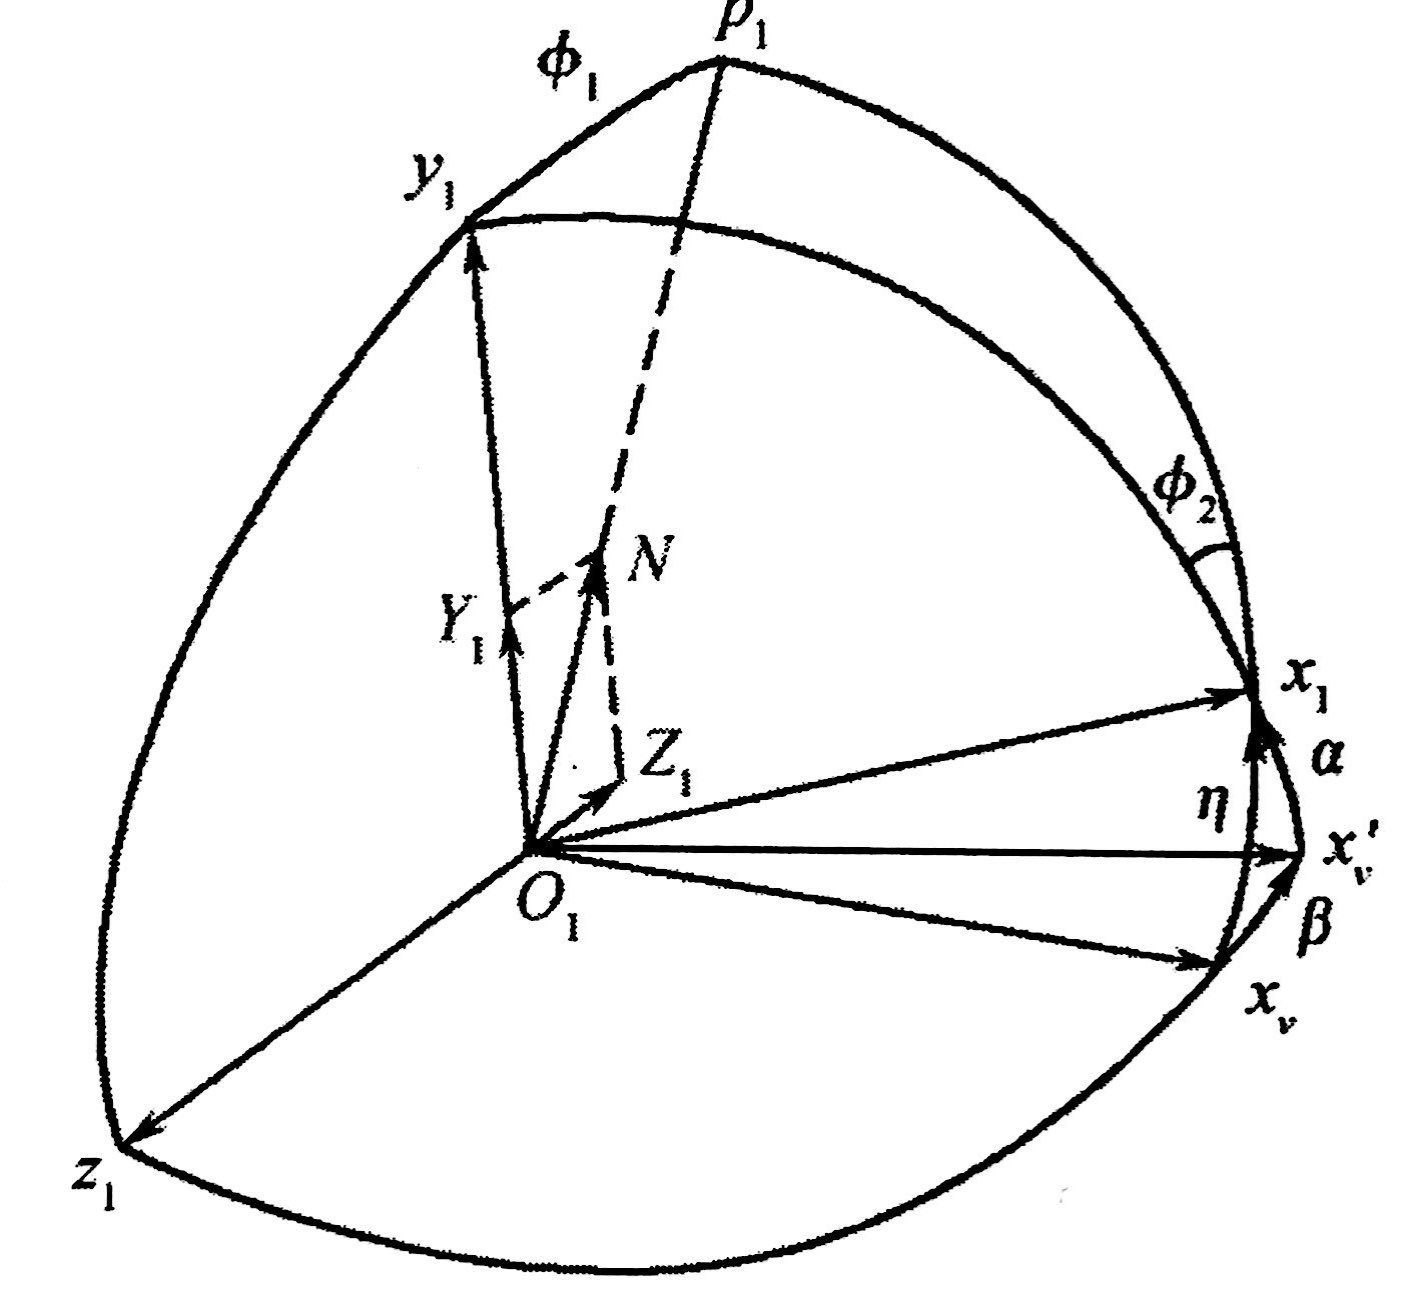
\includegraphics[width=0.4\linewidth]{pic/总法向力.jpg}
	\caption{总法向力$N$与法向力$Y_1$、横向力$Z_1$之间的关系}
\end{figure}
\vspace*{-1em}
\begin{equation}
	N \bm{n}^0 = Y_1\bm{y_1}^0 + Z_z \bm{z}_1^0 \qquad 
	\begin{cases}
		Y_1 = N \cos \phi_1 \\
		Z_1 = - N \sin \phi_1 
	\end{cases}
	\qquad 
	N^2 = Y_1^2 + Z_1^2
\end{equation}
\par 根据球面三角形公式,因为$o_1x_1$垂直于$y_1o_1p_1$平面,则
\begin{equation}
	\phi_1 = \phi_2
\end{equation}
由于在球面三角形$x_vx'_vx_1$中,$\angle x_vx'_v x_1 = 90 \degree$,所以球面三角形$x_vx'_vx_1$为球面直角三角形,则有
\par \blue[正弦公式]
\begin{equation}
	\sin \phi_2 = \dfrac{\sin \beta}{\sin \eta}
\end{equation}
\par \blue[余弦公式]
\begin{equation}
	\begin{cases}
		\, \cos \phi_2 = \dfrac{\cos \beta - \cos \alpha \cos \eta }{\sin \alpha \sin \eta}\\[0.5em]
		\, \cos \eta = \cos \beta \cdot \cos \alpha
	\end{cases}
	\quad \Rightarrow \quad 
	\cos \phi_2 = \dfrac{\sin \alpha \sin \beta}{\sin \eta}
\end{equation}

因此有法向力、横向力表达式
\begin{equation}
	\begin{cases}
		Y_1 = N \dfrac{\sin \alpha \sin \beta }{\sin \eta }\\[0.8em]
		Z_1 = -N \dfrac{\sin \beta}{\sin \eta}
	\end{cases}
	\qquad
	\begin{cases}
		C_{y1} = C_N \dfrac{\sin \alpha \sin \beta}{\sin \eta}\\[0.8em]
		C_{z1} = - C_N \dfrac{\sin \beta}{\sin \eta}
	\end{cases}
	\qquad
	C_N^2 = C_{y1}^2 + C_{z1}^2
\end{equation}
\vspace*{0.5em}

\noa[4] 总升力$L$与升力$Y$、侧力$Z$的关系
\begin{figure}[!htb]
	\centering
	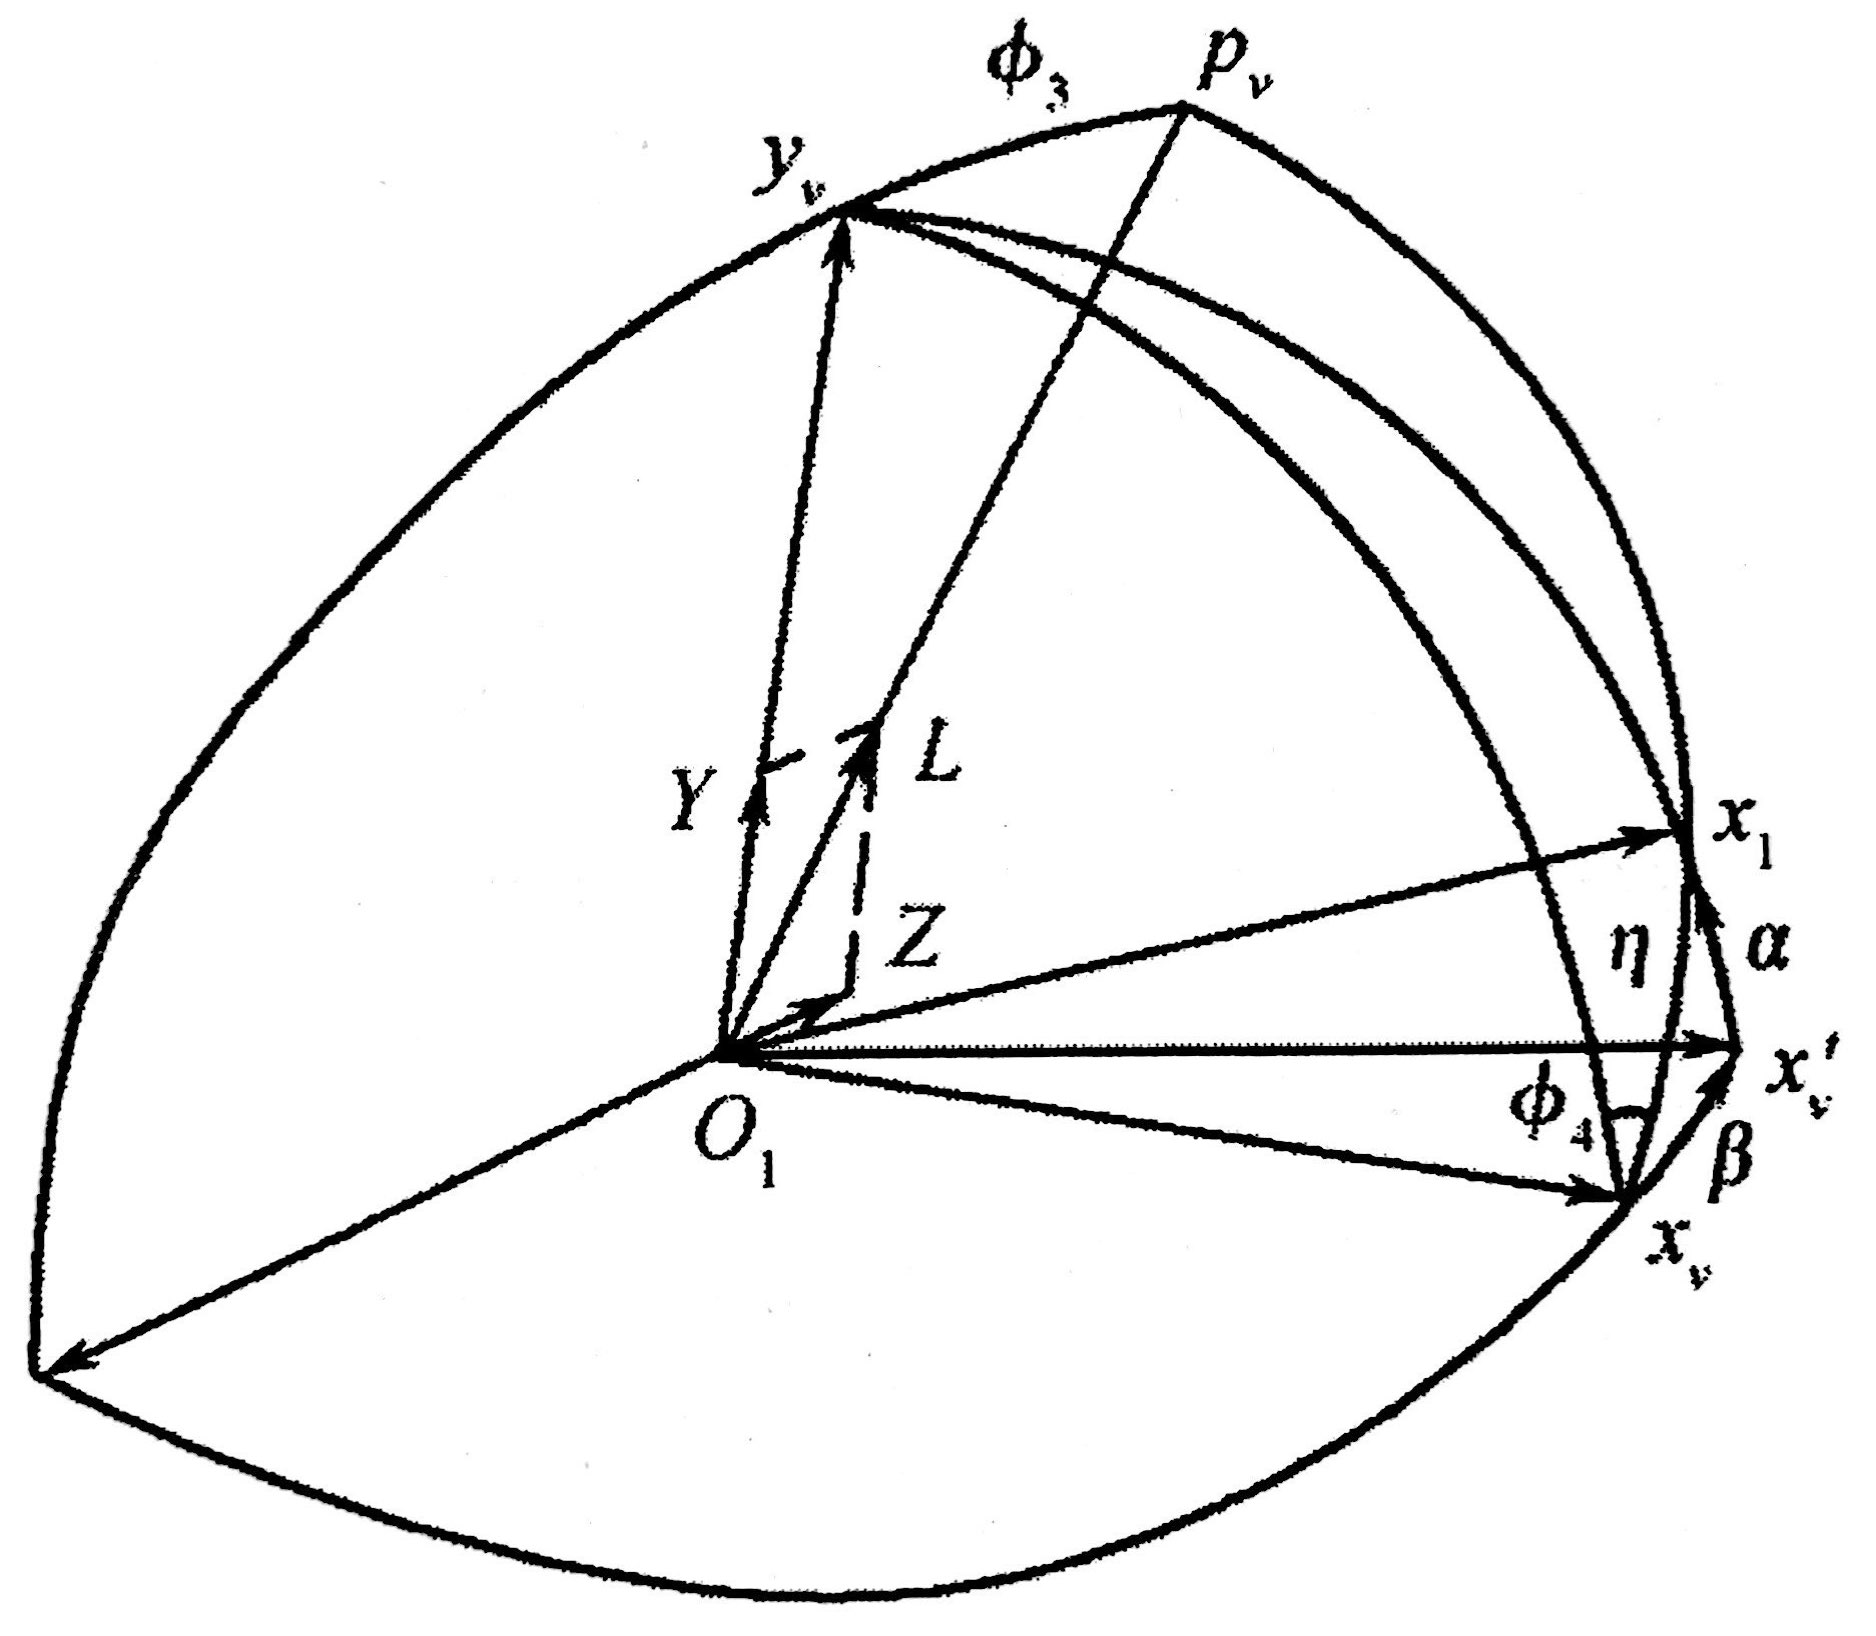
\includegraphics[width=0.4\linewidth]{pic/总升力.jpg}
	\caption{总升力$L$与升力$Y$、侧力$Z$的关系}
\end{figure}
\vspace*{-1em}
\begin{equation}
	L\bm{l}^0 = Y\bm{y}_v^0 + Z\bm{z}_v^0 \qquad 
	\begin{cases}
		\, Y = L \cos \phi_3 \\
		\, Z = - L \sin \phi_3
	\end{cases}
	\qquad 
	L^2 = Y^2 + Z^2
\end{equation}
根据球面三角形公式,有
\begin{equation}
	\phi_3 = \phi_4 = 90\degree - \angle x_1x_vx'_v
\end{equation}
而根据球面直角三角形,有
\begin{align}
	\cos \phi_4 &= \dfrac{\sin \alpha}{\sin \eta} \\[0.5em]
	\sin \phi_4 &= \dfrac{\cos \alpha \sin \beta}{\sin \eta}
\end{align}

因此有升力、侧力表达式为
\begin{equation}
	\begin{cases}
		\, Y = L \dfrac{\sin \alpha}{\sin \eta} \\[0.8em]
		\, Z = - L \dfrac{\cos \alpha \sin \beta}{\sin \eta}
	\end{cases}
	\qquad 
	\begin{cases}
		\, C_y = C_L \dfrac{\sin \alpha }{\sin \eta} \\[0.8em]
		\, C_z = - C_L \dfrac{\cos \alpha \sin \beta}{\sin \eta}
	\end{cases}
	\qquad 
	C_L^2 = C_y^2 + C_z^2
\end{equation}
\vspace*{0.5em}

\noa[4] 气动力$R$在发射系中的描述

\begin{equation}
	\bm{x}_1^0 = \cos \eta \bm{x}_v^0 + \sin \eta \bm{l}^0
\end{equation}
则
\begin{equation}
	\bm{R} = - X \bm{x}_v^0 + L \bm{l}^0 = - X\bm{x}_v^0 + \dfrac{L}{\sin \eta}\big(\bm{x}_1^0 - \cos \eta \bm{x}_v^0\big)
\end{equation}
\begin{figure}[!htb]
	\centering
	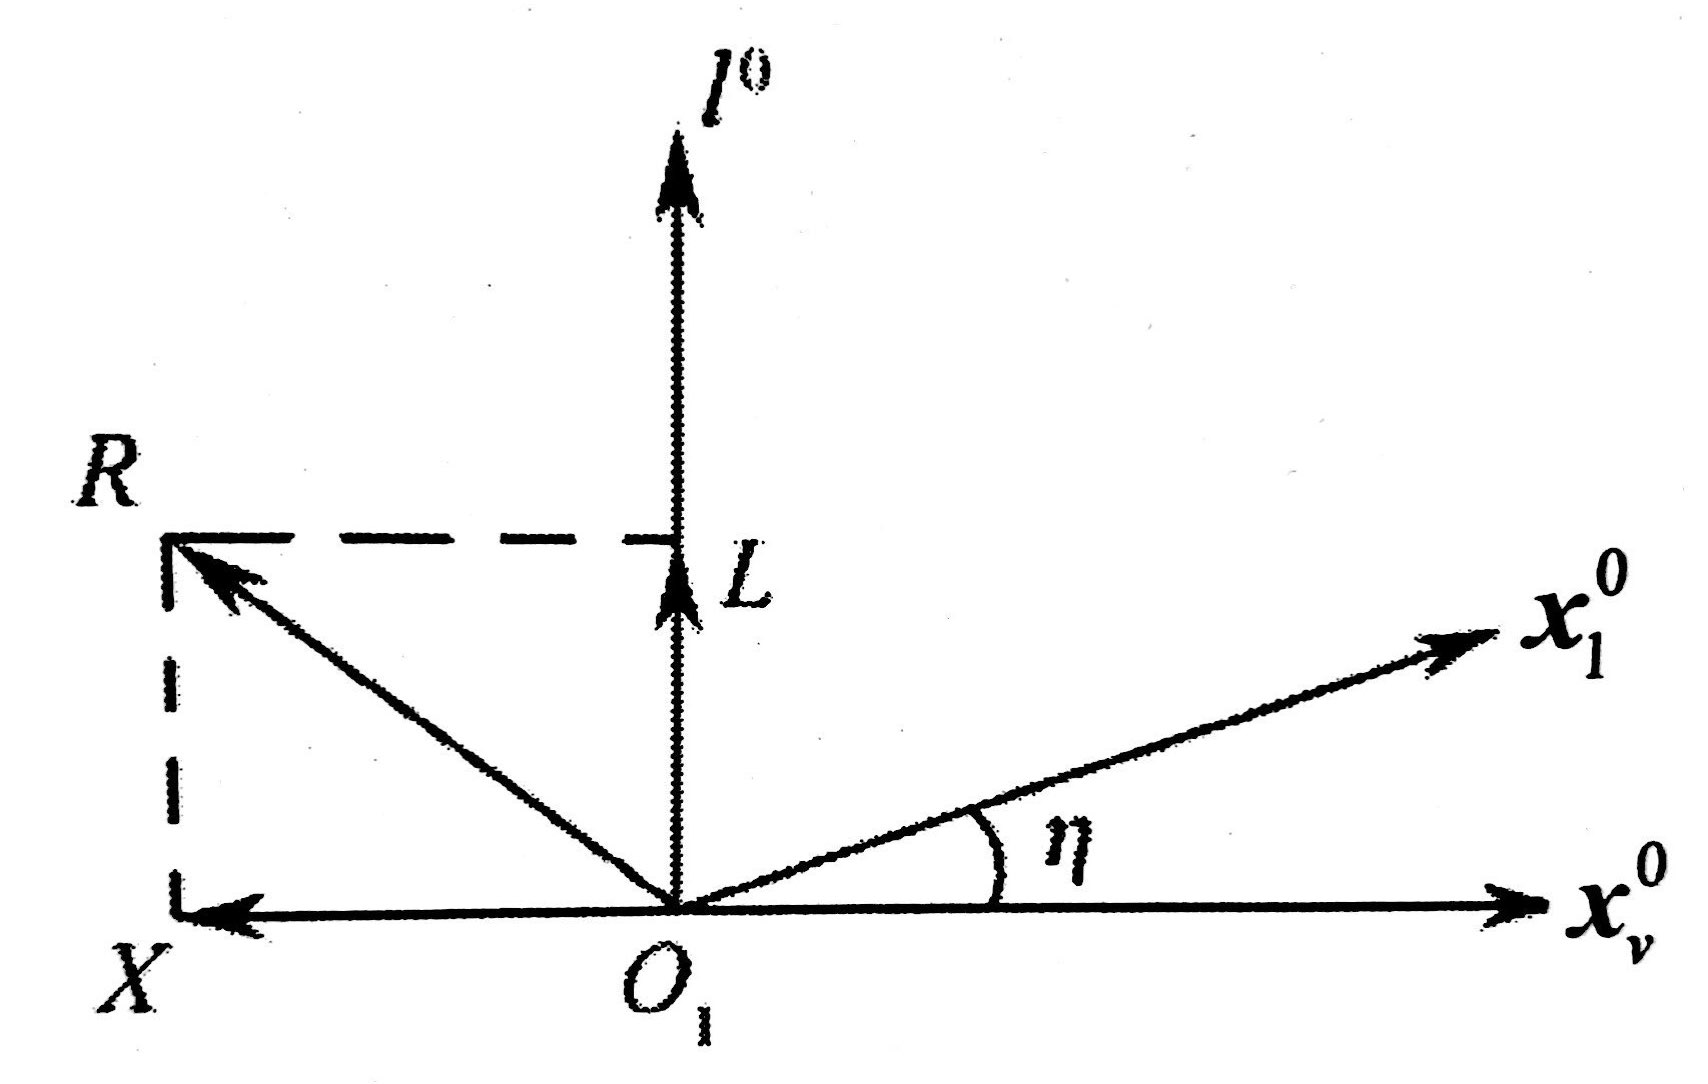
\includegraphics[width=0.4\linewidth]{pic/总气动力.jpg}
	\caption{单位矢量$\bm{l}^0$与$\bm{x}_1^0, \bm{x}_v^0$的关系}
\end{figure}

利用箭体系与发射系的方向余弦矩阵$\bm{G}_B$,有
\begin{equation}
	\bm{R} = 
	\begin{bmatrix}
		R_x \\
		R_y\\
		R_z
	\end{bmatrix}
	= -X
	\begin{bmatrix}
		\cos \theta \cos \sigma \\
		\sin \theta \cos \sigma \\
		- \sin \sigma
	\end{bmatrix}
	+ \dfrac{L}{\sin \eta}
	\begin{bmatrix}
		\cos \varphi \cos \psi - \cos \psi \cos \theta \cos \sigma \\
		\sin \varphi \cos \psi - \cos \eta \sin \theta \cos \sigma\\
		- \sin \psi + \cos \eta \sin \sigma
	\end{bmatrix}
\end{equation}
进一步可利用速度分解量简化计算,有
\begin{equation}
	\bm{v} = 
	\begin{bmatrix}
		v_x \\
		v_y \\
		v_z
	\end{bmatrix}
	= 
	-v
	\begin{bmatrix}
		\cos \theta \cos \sigma \\
		\sin \theta \cos \sigma \\
		- \sin \sigma 
	\end{bmatrix}
	\qquad 
	\bm{R} = -\dfrac{\red[X]}{v}
	\begin{bmatrix}
		v_x \\
		v_y\\
		v_z
	\end{bmatrix}
	+ \dfrac{\red[L]}{v \sin \red[\eta]}
	\begin{bmatrix}
		v \cos \varphi \cos \psi - \cos \red[\eta] v_x \\
		v \sin \varphi \cos \psi - \cos \red[\eta] v_y \\
		- v \sin \psi + \cos \red[\eta] v_z 
	\end{bmatrix}
\end{equation}
\vspace*{0.5em}

\noa[6] 稳定力矩描述

如果飞行器质心与压心均位于纵轴上,有
\begin{equation}
	\bm{M}_{st} = 
	\begin{bmatrix}
		M_{x1st}\\
		M_{y1st}\\
		M_{z1st}
	\end{bmatrix}
	=
	\begin{bmatrix}
		0 \\
		Z_1\big(x_p - x_g\big) \\
		-Y_1 \big(x_p - x_g\big)
	\end{bmatrix}
\end{equation}
代入
\begin{equation*}
	\begin{cases}
		\, Y_1 = N\dfrac{\sin \alpha \sin \beta}{\sin \eta}\\[0.8em]
		\, Z_1 = - N \dfrac{\sin \beta}{\sin \eta}
	\end{cases}
\end{equation*}
则
\begin{equation}
	\bm{M}_{st} = 
	\begin{bmatrix}
		M_{x1st}\\
		M_{y1st}\\
		M_{z1st}
	\end{bmatrix}
	=
	\begin{bmatrix}
		0 \\
		- m_n q S_M l_k \dfrac{\sin \beta}{\sin \eta} \\[0.8em]
		- m_n q S_M l_k \dfrac{\sin \alpha \cos \beta}{\sin \eta}
	\end{bmatrix}
\end{equation}
其中,$m_n = C_N \big(\overline{x}_p - \overline{x}_g\big)$为\dy[稳定力矩系数]{WDLJXS}。


\subsection{简化的再入段平面运动方程}

考虑到再入飞行器特别是弹头的射程较小,飞行时间较短,因此在研究其运动时可假设

\noa[1] 不考虑地球自转,即$\omega_e = 0$。

\noa[2] 认为地球为均质圆球,引力场为有心力场。

\noa[3] 认为飞行器纵轴始终处于再入射面内,即侧滑角为0。

建立再入坐标系$e-xyz$,$e-xy$面即为再入射面。

\begin{figure}[!htb]
	\centering
	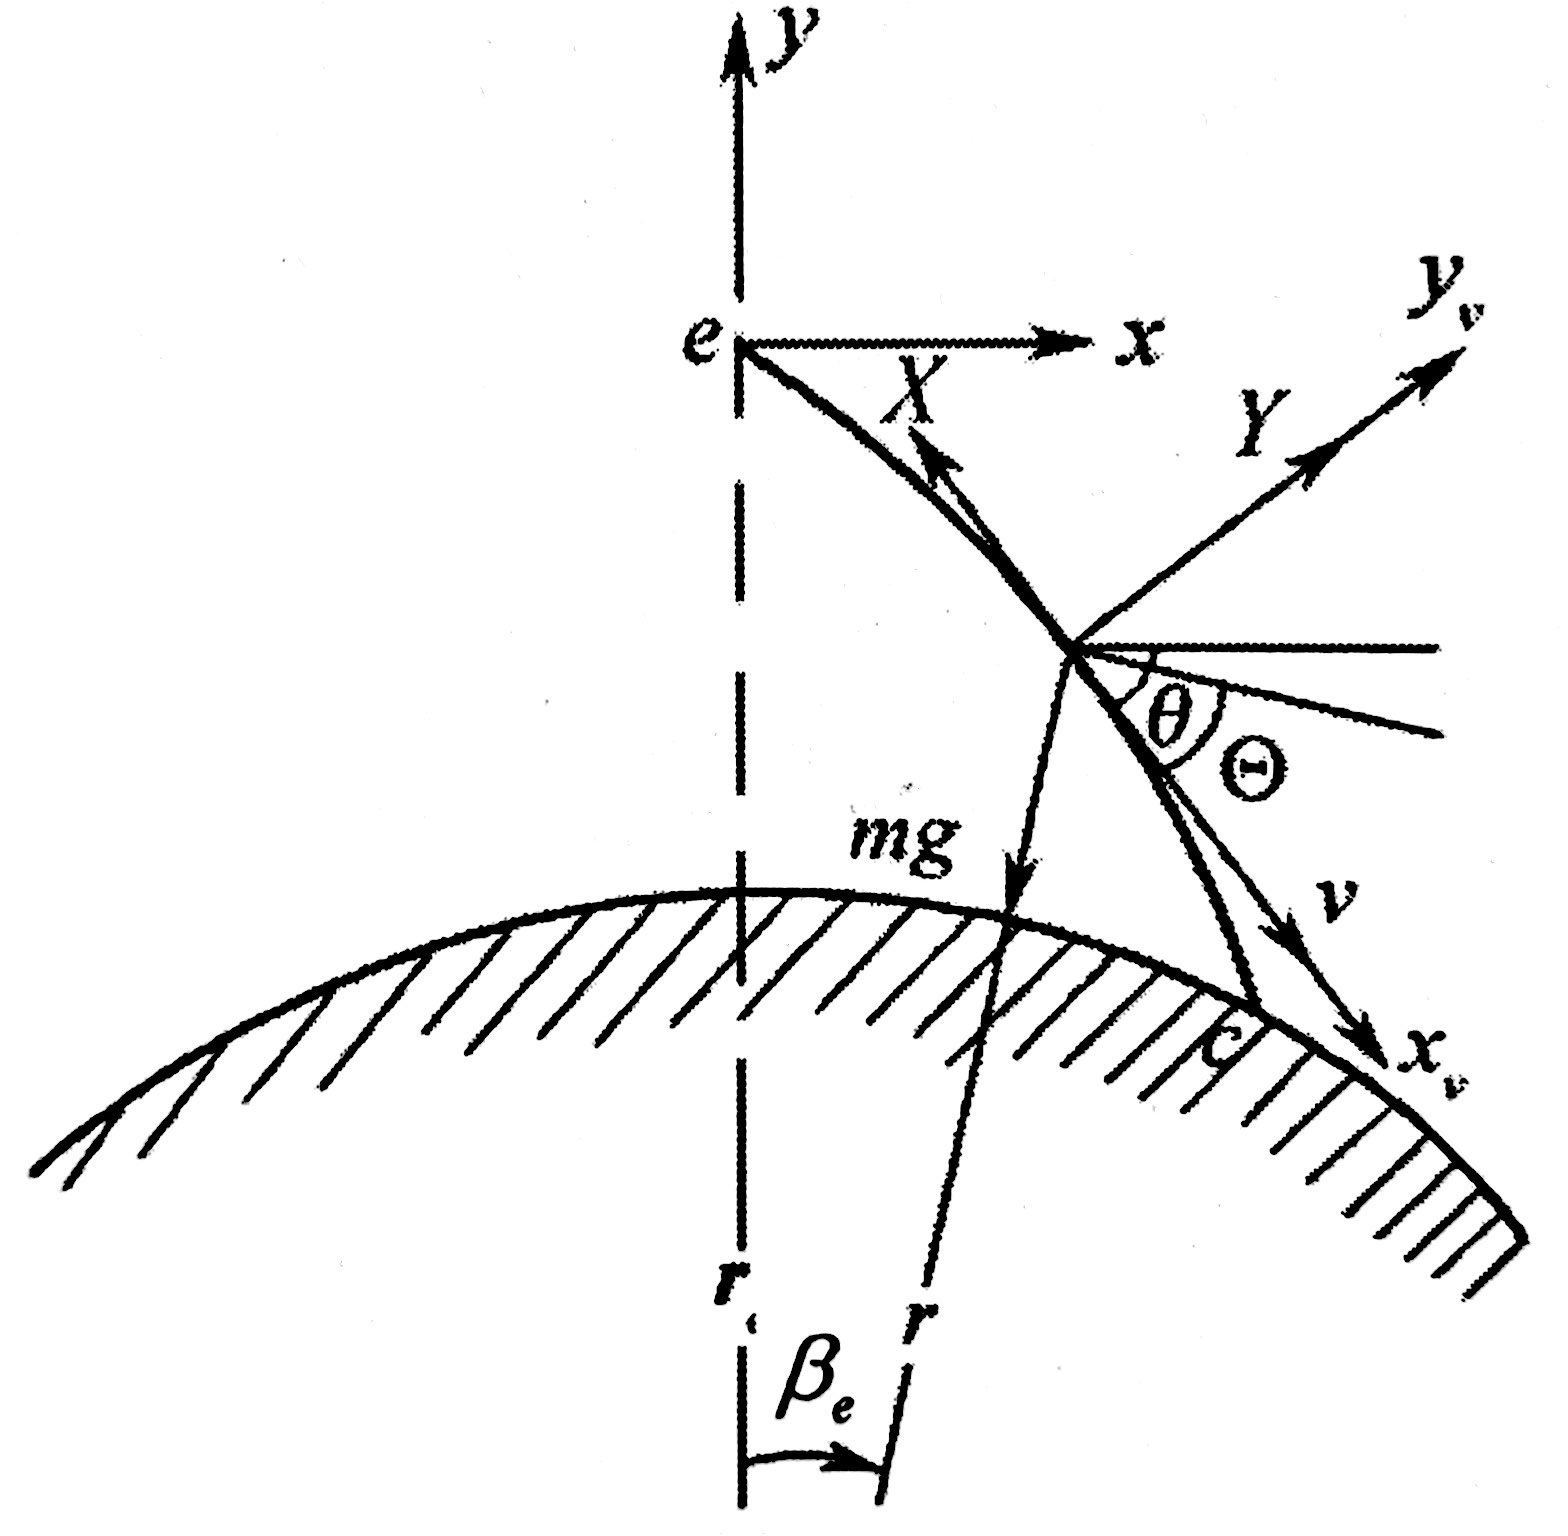
\includegraphics[width=0.3\linewidth]{pic/再入段坐标系与力.jpg}
	\caption{再入段坐标系与力}
\end{figure}
再入状态变量:速度、当地速度倾角、地心距、再入段射程角。

再入矢量方程为
\begin{equation}
	\dfrac{\d \bm{v}}{\d t} = \bm{R} + m \bm{g}
\end{equation}
将运动方程投影到速度系中, 有
\begin{equation}
	\dfrac{\d \bm{v}}{\d t} = \dfrac{\d v}{\d t}\bm{x}_v^0 + v \dfrac{\d \theta}{\d t} \bm{y}_v^0
\end{equation}
代入具体的气动力及引力,有
\begin{equation}
	\begin{cases}
		\, \dfrac{\d v}{\d t} = - \dfrac{X}{m} - g \sin \varTheta \\[0.5em]
		\, \dfrac{\d \theta}{\d t} = \dfrac{Y}{m v} - \dfrac{g}{v} \cos \varTheta
	\end{cases}
\end{equation}
速度倾角之间的关系有
\begin{align}
	\varTheta = \theta + \beta_e \\
	\dot{\varTheta} = \dot{\theta} + \dot{\beta}_e
\end{align}
而速度在地心距及当地水平方向的投影为
\begin{equation}
	\begin{cases}
		\, \dot{r} = v \sin \varTheta \\
		\, r \dot{\beta}_e = v \cos \varTheta
	\end{cases}
\end{equation}
则有
\begin{equation}
	\dot{\varTheta} = \dot{\theta} + \dot{\beta}_e = \dfrac{Y}{m v} - \dfrac{g}{v}\cos \varTheta + \dfrac{v}{r}\cos \varTheta
\end{equation}
则简化后的再入平面运动方程为
\begin{equation}
	\begin{cases}
		\, \dot{v} = - \dfrac{X}{m} - g \sin \varTheta \\[0.5em]
		\, \dot{\varTheta} = \dfrac{Y}{mv} + \left(\dfrac{v}{r} - \dfrac{g}{v}\right)\cos \varTheta
	\end{cases}
	\qquad 
	\begin{cases}
		\, \dot{r} = v \sin \varTheta \\
		\, \dot{\beta}_e = \dfrac{v}{r} \cos \varTheta
	\end{cases}
\end{equation}

质心方程中气动力计算与攻角有关,不能直接求解,需要补充姿态方程:
\begin{equation}
	\begin{cases}
		I_{z1} \dfrac{\d \omega_{z1}}{\d t} = m_{z1}^{\overline{\omega}}qS_ML_k\overline{\omega} + m_{z1\text{st}}qS_ML_k \\[0.5em]
		\dfrac{\d \varphi}{\d t} = \omega_{z1} \\
		\alpha = \varphi - \theta = \varphi + \beta_e - \varTheta
	\end{cases}
\end{equation}

一般来说,飞行器是以任意姿态进入大气层的,其运动包含质心运动和绕质心运动。对于静稳定的再入飞行器,当有攻角时,稳定力矩将使其减小,飞行器会很快稳定下来。此时\red[总攻角]为零,飞行器不受升力作用,称为\dy[弹道再入]{DDZR}或\dy[零升力再入]{LSLZR}、\dy[零攻角再入]{LGJZR}。反之,如果再入过程中总攻角不为零,飞行器受升力作用,其再入称为\dy[有升力再入]{YSLZR}。







\section{零攻角再入弹道特性分析}

无论采用何种再入方式,用计算机\red[数值积分]均可得到再入弹道参数。但在初步设计中,希望快速求得飞行器运动参数,并分析各种因素对运动参数的影响,如弹头结构承受的\red[最大过载]、\red[热流]及\red[烧蚀]等,因此需要相关参数的\red[近似解析解]。一般采用简化的平面运动方程。

对于零攻角再入,升力为零,有

\theorem[零攻角再入平面运动方程]
{
	\vspace*{-1em}
	\begin{equation}
		\begin{cases}
			\, \dot{v} = \dfrac{X}{m} - g \sin \varTheta \\
			\, \dot{\varTheta} = \left(\dfrac{v}{r} - \dfrac{g}{v}\right) \cos \varTheta \\
			\, \dot{r} = v \sin \varTheta \\
			\, \dot{\beta}_e = \dfrac{v}{r} \cos \varTheta
		\end{cases}
	\end{equation}
	对于速度方程,代入气动力表达式,可以得到
	\begin{equation}
		\dfrac{\d v}{\d t} = - C_x \dfrac{\rho v^2 S}{2 m} - g \sin \varTheta
	\end{equation}
	为了得到近似解,需对地球大气进行假设
	\begin{equation}
		\rho = \rho_0 \cdot \e^{- \beta h}, \qquad \beta = \dfrac{1}{7200} (\text{m}^{-1})
	\end{equation}
	并以\red[高度]为\red[自变量]
	\begin{equation}
		\d t = \dfrac{\d h}{v \sin \varTheta}
	\end{equation}
}


\subsection{再入段最小负加速度的近似计算}

飞行器高速进入稠密大气时,空气阻力使飞行器减速,其阻力加速度可达几十个$g$,使弹头结构及仪表工作受到很大影响。因此\red[最小负加速度]是初步设计必须考虑的问题。最小负加速度也可称为\dy[最大过载]{ZDGZ}。

进一步假设:

\noa[1] \red[忽略地球引力]作用,再入弹道为\red[直线弹道]。因为除再入初始段外,气动阻力远远大于引力值。

\noa[2] 当地水平线转动角速度为零,\red[当地速度倾角]不变。因为再入射程很短,可以将\red[地球看成平面]。

\noa[3] \red[阻力系数为常数]。因为在最大过载前,飞行速度很大,阻力系数很小。

\dy[再入负加速度]{ZRFJSD}\quad 再入时受到气动力作用,若为零攻角再入则表示为阻力,产生的气动力很大,且为负加速度。

由动力学方程可得
\begin{equation}
	\begin{cases}
		\, \dot{v} = - \dfrac{X}{m} = \dfrac{C_x \rho_0 S_M}{2 m} \e^{- \beta h} v^2 \\[0.5em]
		\, \dot{h} = v \sin \varTheta_e
	\end{cases}
\end{equation}
引入\dy[弹道系数]{DDXS}
\begin{equation}
	B = \dfrac{C_x S_M}{2 m}
\end{equation}
速度方程变为
\begin{equation}
	\dfrac{\d v}{\d h} = - \dfrac{B \rho_0}{\sin \varTheta_e}\e^{-\beta h}v \qquad \dfrac{\d v}{v} = \dfrac{B \rho_0}{\beta \sin \varTheta_e}\e^{-\beta h} \d \big(- \beta h\big)
\end{equation}
假设再入点大气密度为零,则有速度表达式为
\begin{equation}
	v = v_e \exp \left(\dfrac{B \rho_0}{\beta \sin \varTheta_e} \e ^{- \beta h}\right)
	\label{vh}
\end{equation}

由$\dfrac{\d \dot{v}}{\d h} = 0$可得最大过载发生高度为
\begin{equation}
	\begin{cases}
		\, \dot{v} = \dfrac{C_x \rho_0 S_M}{2m}\e^{-\beta h}v^2 \\[0.5em]
		\, \dfrac{\d v}{\d h} = - \dfrac{B \rho_0}{\sin \varTheta_e}\e^{-\beta h}v
	\end{cases}
	\quad \Rightarrow \quad 
	\dfrac{\d \dot{v}}{\d h} = B \rho v^2 \left(\beta + \dfrac{2B\rho}{\sin \varTheta_e}\right) = 0 \quad \Rightarrow \quad \rho_m\big(h_m\big) = - \dfrac{\beta \sin \varTheta_e}{2 B}
\end{equation}
则

\theorem[最大过载的计算]
{
	\textbf{\dy[最大过载发生高度]{ZDGZFSGD}}
	\begin{equation}
		h_m = \dfrac{1}{\beta} \ln \left(- \dfrac{2B\rho_0}{\beta \sin \varTheta_e}\right) = \dfrac{1}{\beta}\ln \left(- \dfrac{C_xS_M \rho_0}{m \beta \sin \varTheta_e}\right)
	\end{equation}
\blue[最大过载发生高度与质量、尺寸、倾角有关,但与速度无关。]\\[0.5em]
	\hspace*{2em} \textbf{\dy[最大过载速度]{ZDGZSD}}
	\begin{equation}
		v_m = v_e \exp \left(\dfrac{B \rho_m}{\beta \sin \varTheta_e}\right) = v_e \e^{-0.5} \approx 0.61 v_e
	\end{equation}
\blue[最大过载速度只与速度有关,与质量、尺寸、倾角无关。]\\[0.5em]
\hspace*{2em} \textbf{\dy[最大过载]{ZDGZ}}
\begin{equation}
	\dot{v}_{\min} = - B \rho_m v_m^2 = \dfrac{\beta v_e^2}{2 e}\sin \varTheta_e
\end{equation}
\blue[最大过载只与速度、倾角有关,与质量、尺寸无关。]
}


\subsection{热流的近似计算}

巨大的飞行器机械能通过大气阻力转变为热能,使大气温度上升至几千度。因此需要对热流进行计算,以保证弹体结构防热安全。

热流主要考虑三个参数:\dy[平均对流热流$q_{av}$]{PJDLRL};\dy[驻点对流热流$q_s$]{ZDDLRL};\dy[总吸热量$Q$]{ZXRL}。
\vspace*{0.5em}

\sssection[平均热流$q_{av}$]

平均热流的定义式为
\begin{equation}
	q_{av} = \dfrac{1}{S_T}\int_s q\, \d s = \dfrac{1}{4} C'_f\rho v^3
\end{equation}
代入速度表达式
\begin{equation}
	v = v_e \exp\left(\dfrac{B \rho_0}{\beta \sin \varTheta} \e^{- \beta h}\right)
\end{equation}
可以得到
\begin{equation}
	q_{av} = \dfrac{1}{4}C'_f \rho v_e^3 \exp\left(\dfrac{3B}{\beta \sin \varTheta}\rho \right)
\end{equation}
对大气密度进行求导,并令其导数为零,则有
\begin{align}
	\rho_{m1} &= -\dfrac{\beta \sin \varTheta_e}{3 B} \label{qav1}\\[0.5em]
	h_{m1} = \dfrac{1}{\beta}\ln \left(- \dfrac{3B\rho_0}{\beta \sin \varTheta_e}\right) &= \dfrac{1}{\beta} \ln \left(- \dfrac{3C_x S_M \rho_0}{2 m \beta \sin \varTheta_e}\right) \qquad \mbox{与速度无关}
\end{align}
由速度与高度关系 \eqref{vh} 及密度公式 \eqref{qav1},可以计算得到

\theorem[最大平均热流]
{
	\textbf{\dy[最大平均热流点速度]{ZDPJRLDSD}}
	\begin{equation}
		v_{m1} = v_e \exp\left(\dfrac{B \rho_{m1}}{\beta \sin \varTheta_e}\right) = v_e \e^{-\textstyle \frac{1}{3}} \approx 0.72v_e
	\end{equation}
	\blue[最大过载发生高度只与速度有关,与质量、尺寸、倾角无关。]\\[0.5em]
	\hspace*{2em} \textbf{\dy[最大平均热流]{ZDPJRL}}
	\begin{equation}
		\big(q_{av}\big)_{\max} = - \dfrac{1}{12}C'_f v_e^3 \dfrac{\beta \sin \varTheta_e}{B \cdot \e}
	\end{equation}
}


\sssection[驻点热流$q_s$]

驻点热流的定义式为
\begin{equation}
	q_{s} = k_s \sqrt{\rho}\cdot v^3
\end{equation}
代入速度表达式
\begin{equation}
	v = v_e \exp\left(\dfrac{B \rho_0}{\beta \sin \varTheta} \e^{- \beta h}\right)
\end{equation}
可以得到
\begin{equation}
	q_s = k_s \sqrt{\rho}v_e^3\exp\left(\dfrac{3B}{\beta \sin \varTheta} \rho\right)
\end{equation}
对大气密度进行求导,并令其导数为零,则有
\begin{align}
	\rho_{m2} &= -\dfrac{\beta \sin \varTheta_e}{6 B} \label{qs1}\\[0.5em]
	h_{m2} = \dfrac{1}{\beta}\ln \left(- \dfrac{6B\rho_0}{\beta \sin \varTheta_e}\right) &= \dfrac{1}{\beta} \ln \left(- \dfrac{3C_x S_M \rho_0}{m \beta \sin \varTheta_e}\right) \qquad \mbox{与速度无关}
\end{align}
由速度与高度关系 \eqref{vh} 及密度公式 \eqref{qs1},可以计算得到

\theorem[最大驻点热流]
{
	\textbf{\dy[最大平均热流点速度]{ZDPJRLDSD}}
	\begin{equation}
		v_{m2} = v_e \exp\left(\dfrac{B \rho_{m2}}{\beta \sin \varTheta_e}\right) = v_e \e^{-\textstyle \frac{1}{6}} \approx 0.85v_e
	\end{equation}
	\blue[最大过载发生高度只与速度有关,与质量、尺寸、倾角无关。]\\[0.5em]
	\hspace*{2em} \textbf{\dy[最大平均热流]{ZDPJRL}}
	\begin{equation}
		\big(q_{s}\big)_{\max} = ks v_e^3 \sqrt{\dfrac{-\beta \sin \varTheta_e}{6B\cdot \e}}
	\end{equation}
}

\sssection[总吸热量$Q$]

总吸热量的定义为平均热流的时间积分,即
\begin{equation}
	Q = \int_0^t q_{av} S_T \,\d t = \dfrac{C'_f S_T}{4} \int_0^t \rho v^3 \, \d t
\end{equation}
将时间积分转换为大气密度积分后有
\begin{equation}
	\begin{cases}
		\, \d h = v \sin \varTheta_e \, \d t \\
		\, \d \rho = - \beta \rho \, \d h
	\end{cases}
	\quad \Rightarrow \quad \d t = -\dfrac{1}{\beta \rho v \sin \varTheta_e}\, \d \rho \quad \Rightarrow \quad 
	Q = - \int_{\rho_e}^{\rho} \dfrac{C'_f S_T}{4 \beta \sin \varTheta_e} v^2 \, \d \rho
\end{equation}
代入速度表达式 \eqref{vh} ,并积分后得
\begin{equation}
	\begin{split}
		Q &= \dfrac{C'_fS_T}{8B}v_e^2 \Bigg[\exp\left(\dfrac{2B\rho_0 \e^{-\beta h_e}}{\beta \sin \varTheta_e}\right) - \exp \left(\dfrac{2B \rho_0 \e^{-\beta h}}{\beta \sin \varTheta_e}\right)\Bigg]\\[0.8em]
		&= \dfrac{C'_fS_T}{8B}v_e^2 \Bigg[1 - \exp \left(\dfrac{2B\rho_0}{\beta \sin \varTheta_e}\right)\Bigg]
	\end{split}
\end{equation}
令
\begin{equation*}
	v_c = v_e \exp\left(\dfrac{B \rho_0}{\beta \sin \varTheta_e}\right)
\end{equation*}
则有

\theorem[总吸热量]
{
	\vspace*{-1em}
\begin{equation}
	Q = \dfrac{C'_fS_T}{8B}v_e^2 \Bigg[1 - \exp \left(\dfrac{2B\rho_0}{\beta \sin \varTheta_e}\right)\Bigg] = \dfrac{C_f' S_T}{8B}\big(v_e^2 - v_c^2\big)
\end{equation}
}



\subsection{运动参数的近似计算}
\sssection[速度与当地速度倾角的近似计算]
\vspace*{-0.5em}

\theorem[动量矩定理]
{
	\index{DLJDL@动量矩定理}质点相对固定点的\blue[动量矩]对时间的一阶导数等于作用于质点上的力对同一点的\blue[力矩]。
}

再入飞行器相对于地球质心利用动量矩定理,则有:
\begin{equation}
	\dfrac{\d }{\d t}\big(r v \cos \varTheta\big) = - r \dfrac{X}{m}\cos \varTheta = - r\dfrac{C_x S_M}{2m}\rho v^2 \cos \varTheta
\end{equation}
由$\dfrac{\d h}{\d t} = v \sin \varTheta$代入可得
\begin{equation}
	\dfrac{\d}{\d h}\big(rv \cos \varTheta\big) = - rv\cos \varTheta\dfrac{C_x S_M}{2 m \sin \varTheta}\rho
\end{equation}
令
\begin{equation}
	k = \dfrac{C_x S_M}{2 m \sin \varTheta}
\end{equation}
则
\begin{equation}
	\dfrac{\d}{\d h}\big(rv \cos \varTheta\big) = - rv\cos \varTheta\dfrac{C_x S_M}{2 m \sin \varTheta}\rho \quad \Rightarrow \quad \dfrac{\d \big(rv \cos \varTheta\big)}{r v \cos \varTheta} = - k \rho \, \d h = - k \rho_0 \e^{- \beta h}\, \d h
\end{equation}
积分后得
\begin{equation}
	\ln \dfrac{rv \cos \varTheta}{r_e v_e \cos \varTheta_e} = \dfrac{k \rho_0}{\beta}\big(\e^{-\beta h} - \e^{- \beta h_e}\big)
\end{equation}
即
\begin{equation}
	rv \cos \varTheta = r_e v_e \cos \varTheta_e \exp \bigg[\dfrac{k}{\beta} \big(\rho - \rho_e\big)\bigg]
\end{equation}
由于再入段处大气仍然稀薄,可以认为是真空,即$\rho_e = 0$,即
\begin{equation}
	r v \cos \varTheta = r_e v_e \cos \varTheta_e \e^{{\textstyle \frac{k}{\beta}} \rho}
\end{equation}

\theorem[动量矩守恒]
{
	若再入段处于真空段时,即$\rho = 0$,则
	\begin{equation}
		r_v \cos \theta = r_e v_e \cos \varTheta_e
	\end{equation}
	即再入段仍然是椭圆轨道上的一部分,满足动量矩守恒。而对于非真空段来说,引入了一个修正系数$\e^{{\textstyle \frac{k}{\beta}}\rho}$,即
	\begin{equation}
		r_v \cos \theta = r_e v_e \cos \varTheta_e\e^{{\textstyle \frac{k}{\beta}}\rho}
		\label{再入动量矩}
	\end{equation}
}

由于公式 \eqref{再入动量矩} 有三个未知数:$r,v,\varTheta$,需要补充一个关系式。以$r$为自变量,对动量矩求$t$的微分
\begin{equation}
	\dfrac{\d }{\d t} \big(rv \cos \varTheta\big) = v \dfrac{\d }{\d t}\big(r \cos \varTheta\big) + r \cos \varTheta \dfrac{\d v}{\d t}
\end{equation}
将$\dfrac{\d v}{\d t} = - \dfrac{X}{m} - g_0 \sin \varTheta$代入,可得
\begin{equation}
	\dfrac{\d }{\d t}\big(r v \cos \varTheta\big) = v \dfrac{\d }{\d t}\big(r \cos \varTheta\big) - r \dfrac{X}{m}\cos \varTheta - rg_0 \sin \varTheta \cos \varTheta
\end{equation}
由动量矩定理,
\begin{equation*}
		\dfrac{\d }{\d t}\big(r v \cos \varTheta\big) = - r \dfrac{X}{m}\cos \varTheta 
\end{equation*}
可以得到
\begin{equation}
	\begin{cases}
		\, v \dfrac{\d }{\d t}\big(r \cos \varTheta\big) = r g_0 \sin \varTheta \cos \varTheta\\[0.5em]
		\, \dfrac{\d h}{\d t} = v \sin \varTheta
	\end{cases}
	\quad \Rightarrow \quad 
	\dfrac{\d \big(r \cos \varTheta\big)}{r \cos \varTheta} = \dfrac{g_0}{v^2}\, \d h
\end{equation}
结合公式 \eqref{再入动量矩} ,可得
\begin{equation}
	\begin{cases}
		\, \dfrac{\d \big(r \cos \varTheta\big)}{r \cos \varTheta} = \dfrac{g_0}{v^2}\, \d h \\[0.5em]
		\, r_v \cos \theta = r_e v_e \cos \varTheta_e\e^{{\textstyle \frac{k}{\beta}}\rho}
	\end{cases}
	\quad \Rightarrow \quad 
	\dfrac{\d \big(r \cos \varTheta\big)}{r^3 \cos^3 \varTheta} = \dfrac{g_0}{r_e^2v_e^2 \cos^2 \varTheta_e}\e^{-2{\textstyle \frac{k}{\beta}}\rho}\, \d h
	\label{再入指数}
\end{equation}
令指数部分
\begin{equation}
	\eta = - 2 \dfrac{k}{\beta} \rho_0 \e^{-\beta h}
\end{equation}
则
\begin{equation*}
	\d \eta = 2 k \rho_0 \e^{-\beta h}\, \d h \quad \Rightarrow \quad \d h = - \dfrac{\d \eta}{\beta \eta}
\end{equation*}
代入公式 \eqref{再入指数} 可得
\begin{equation*}
	\dfrac{\d \big(r \cos \varTheta\big)}{r^3 \cos^3 \varTheta} = -\dfrac{g_0}{\beta r_e^2v_e^2 \cos^2 \varTheta_e}\cdot \dfrac{\e^\eta}{\eta}\, \d \eta
\end{equation*}
积分后可得
\begin{equation}
	\dfrac{1}{2r_e^2\cos^2 \varTheta_e} - \dfrac{1}{2r^2 \cos^2 \varTheta} = - \dfrac{g_0}{\beta r_e^2v_e^2 \cos^2 \varTheta_e}\cdot \int_{\eta_e}^{\eta} \dfrac{\e^\eta}{\eta}\, \d \eta = \dfrac{g_0}{\beta r_e^2v_e^2 \cos^2 \varTheta_e}\cdot  \Bigg[\int_{0}^{\eta}\dfrac{\e^\eta}{\eta}\, \d \eta - \int_{0}^{\eta_e}\dfrac{\e^\eta}{\eta}\, \d \eta \Bigg]
\end{equation}
令
\begin{equation}
	E(\eta) = \int_0^\eta \dfrac{\e^\eta}{\eta}\, \d \eta
\end{equation}
则
\begin{equation}
	\dfrac{1}{2r_e^2\cos^2 \varTheta_e} - \dfrac{1}{2r^2 \cos^2 \varTheta} = \dfrac{g_0}{\beta r_e^2v_e^2 \cos^2 \varTheta_e}\cdot\big[E(\eta) - E(\eta_e)\big]
\end{equation}
解得
\begin{equation}
	r \cos \varTheta = \dfrac{r_e \cos \varTheta_e}{\sqrt{1 + \dfrac{2g_0}{\beta v_e^2\big[E(\eta) - E(\eta_e)\big]}}}
	\label{r-Theta}
\end{equation}

联立 \eqref{再入动量矩},\eqref{r-Theta} 可解得

\theorem[落点速度倾角和速度的近似计算]
{
	\vspace*{-1em}
	\begin{align}
		\cos \varTheta_c &= \dfrac{r_e \cos \varTheta_e}{R}\dfrac{r_e \cos \varTheta_e}{\sqrt{1 + \dfrac{2g_0}{\beta v_e^2\big[E(\eta) - E(\eta_e)\big]}}} \\[0.5em]
		v_c &= \dfrac{r_e v_e \cos \varTheta_e}{R \cos \varTheta_c}\e^{-\dfrac{\eta_0}{2}}
	\end{align}
}


\sssection[射程的近似计算]

由于再入段射程的变化率可写为
\begin{equation}
	\dfrac{\d L_e}{\d h} = \dfrac{\d L_e}{\d t} \cdot \dfrac{\d t}{\d h}
\end{equation}
由$\dfrac{\d \beta_e}{\d t} = \dfrac{v}{r} \cos \varTheta, \dfrac{\d h}{\d t} = v \sin \varTheta, L_e = R \beta_e$,可得
\begin{equation}
	\dfrac{\d L_e}{\d h} = \dfrac{R}{r} \cot \varTheta
\end{equation}
积分后得
 \begin{equation}
 	L_e = R \int_{h_e}^{h} \dfrac{\cot \varTheta}{R + h} \, \d h
 \end{equation}
由于再入段射程较小,可以近似认为$\varTheta = \varTheta_e$,则
\begin{equation}
	L_e = R \cot\varTheta_e \ln \dfrac{R + h}{R + h_e}
\end{equation}
特别地,当$h = 0$时,得到整个再入段射程为
\begin{equation}
	L_e = R \cot \varTheta_e \ln \dfrac{R}{R + h_e}
\end{equation}

\subsection{气动阻力下的被动段弹道}

在自由段并非绝对真空,也会受到气动阻力作用,且射程越近,弹道高度越低,阻力影响就明显。此时被动段弹道有以下特点:

\noa[1] \textbf{在弹道对应高度点,飞行速度不同}

气动阻力始终使速度减小,而引力做功为零。
\vspace*{0.5em}

\noa[2] \textbf{降弧段弹道比升弧段陡}

速度越小,引力作用越明显。
\vspace*{0.5em}
\clearpage

\noa[3] \textbf{最小速度点不在弹道顶点}

在速度最小点,阻力应与引力分量平衡,即
\begin{equation*}
	X + mg \sin \varTheta = 0
\end{equation*}
因此速度最小点只能出现在降弧段,倾角为负。
\vspace*{0.5em}

\noa[4] \textbf{射程与质量相关}

相同阻力下不同质量引起的加速度不同,减速效果不同,影响到速度倾角大小,因此必然影响射程。


\begin{figure}[!htb]
	\centering
	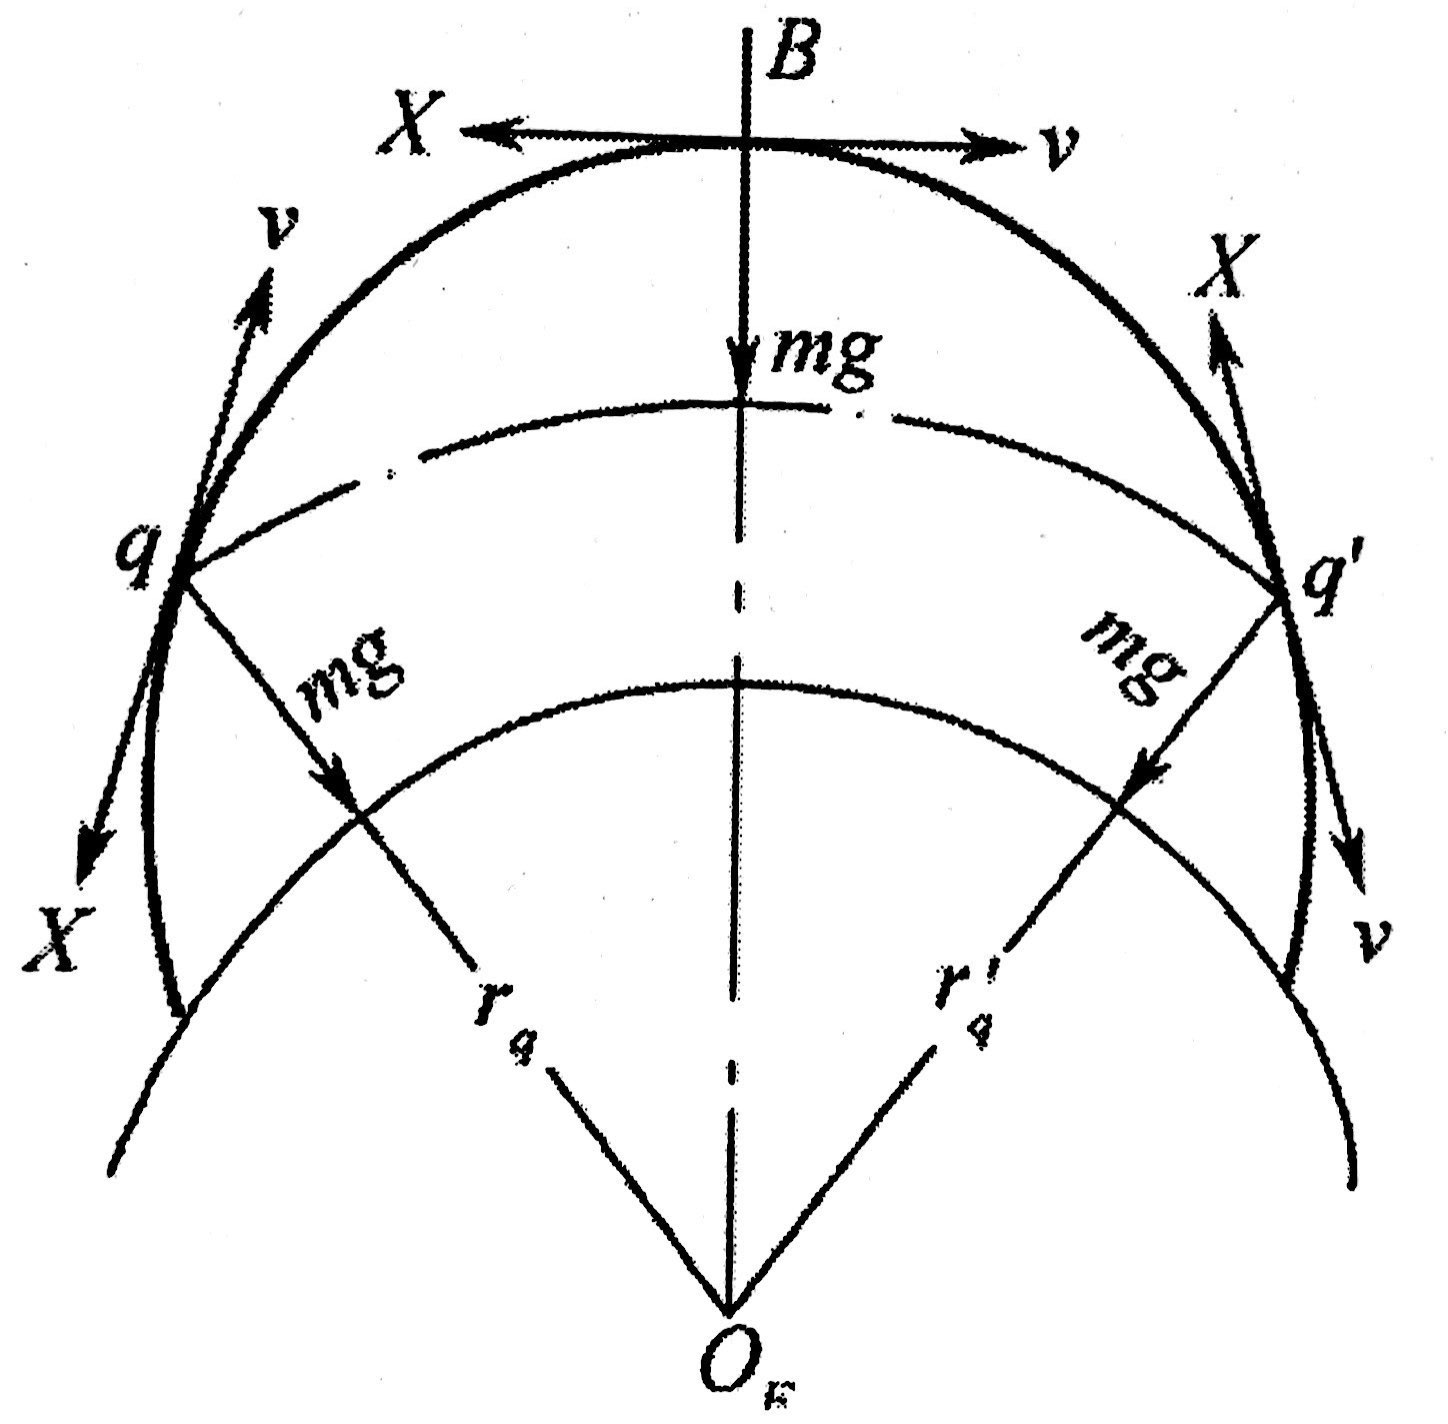
\includegraphics[width=0.35\linewidth]{pic/气动阻力再入.jpg}
	\vspace*{-1em}
	\caption{有空气阻力时被动段弹道各点受力情况}
\end{figure}














